\section{Chi tiết các thành phần bên trong hệ thống}
\label{sec:component-details}
\begingroup
\sloppy

Phần này mô tả chi tiết các thành phần chính của ProLearning Platform theo ba nhóm: \textit{core components}, \textit{support components} và \textit{infrastructure/integration components}. Việc tách nhóm giúp làm rõ thành phần nào trực tiếp tạo ra giá trị học tập cho người dùng, thành phần nào hỗ trợ vận hành nội bộ và thành phần nào phụ trách kết nối hạ tầng hoặc dịch vụ ngoài.

Cách phân nhóm được sử dụng trong báo cáo như sau:

\begin{itemize}
    \item \textbf{Core components:} Bao gồm client, identity, workspace học tập, AI learning, collaboration, review/progress, todo/calendar, pomodoro, notification và payment. Đây là các thành phần trực tiếp tham gia vào trải nghiệm học tập và quản lý tài khoản.
    \item \textbf{Support components:} Bao gồm validation, chuẩn hóa DTO, mapper, xử lý lỗi, phân quyền tài nguyên, cache, scheduler và logging. Đây là các cơ chế dùng chung giúp giảm trùng lặp và tăng tính nhất quán.
    \item \textbf{Infrastructure/integration components:} Bao gồm PostgreSQL, Redis, RabbitMQ, Cloudinary, Firebase Cloud Messaging, Google Calendar, PayOS và SMTP provider. Đây là các thành phần cung cấp năng lực lưu trữ, nhắn tin, đồng bộ và tích hợp ngoài.
\end{itemize}

Hình~\ref{fig:prolearning-architecture-detail-components} mô tả mối quan hệ giữa các nhóm thành phần trên trong kiến trúc hệ thống.

\begin{figure}[htbp]
    \centering
    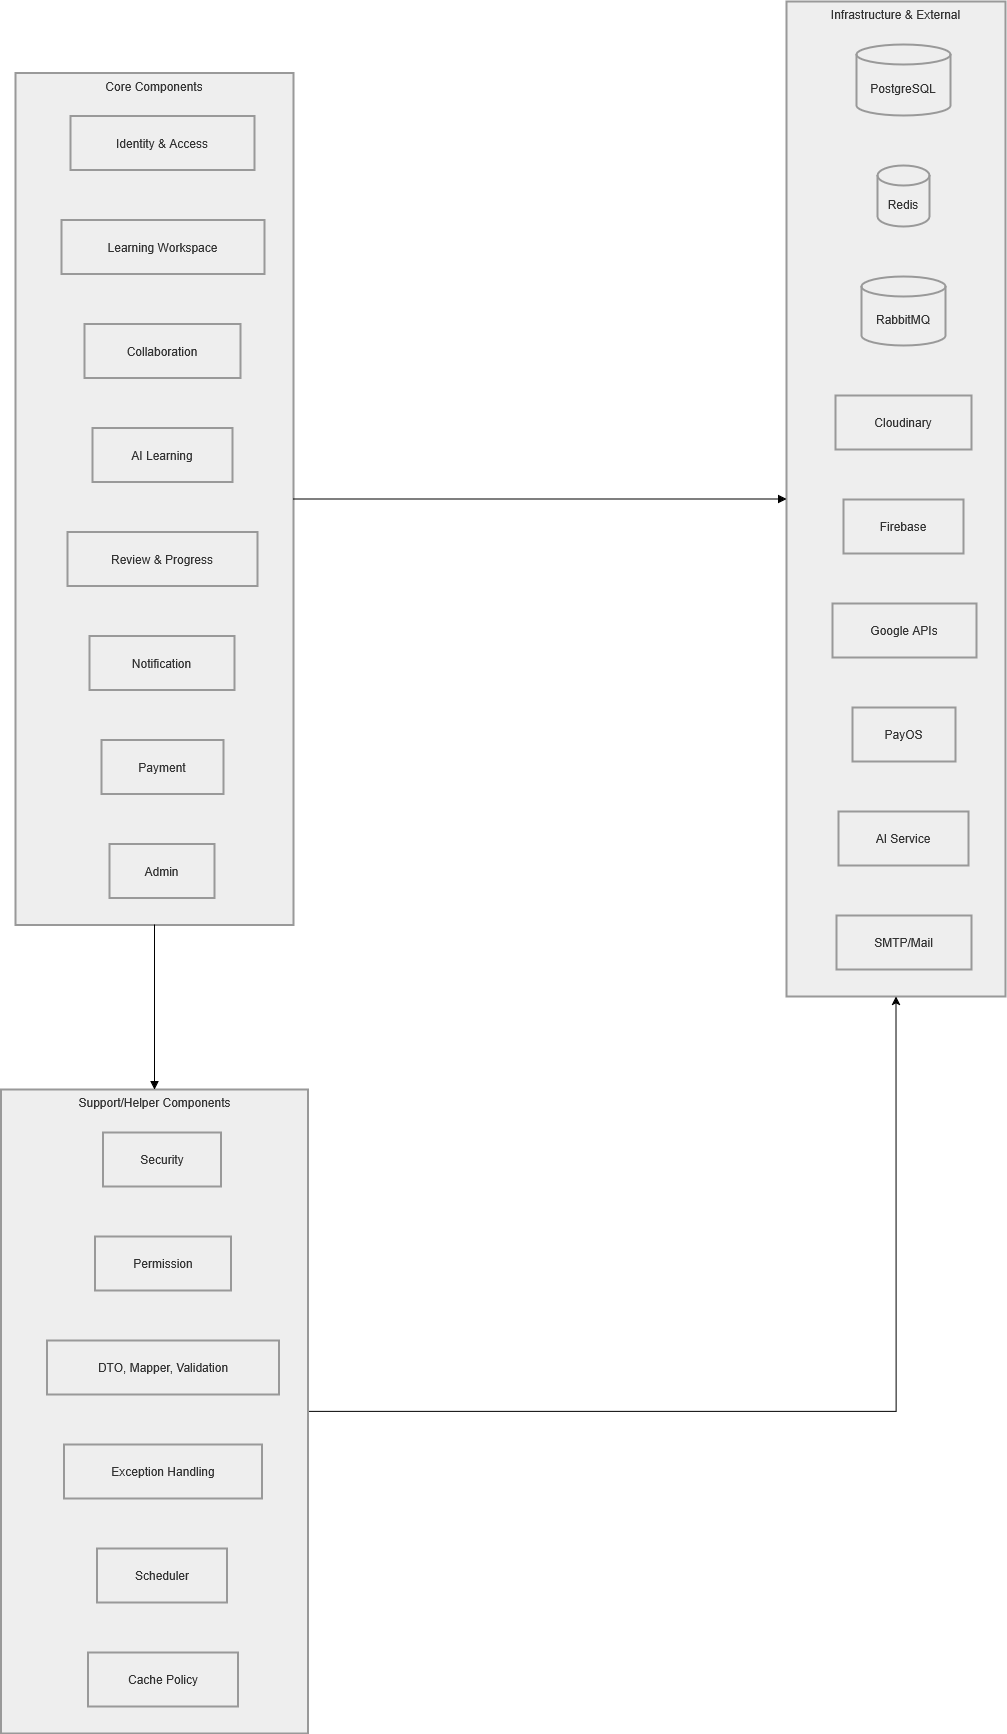
\includegraphics[width=0.95\textwidth,height=0.72\textheight,keepaspectratio]{images/chapter3/ProLearning_Arch-Detail_Components.drawio.png}
    \caption{Chi tiết các thành phần của hệ thống ProLearning Platform}
    \label{fig:prolearning-architecture-detail-components}
\end{figure}

\subsection{Core Components}
\label{subsec:core-components}

Core components là các thành phần trực tiếp phục vụ trải nghiệm học tập và quản lý tài khoản của người dùng. Các thành phần này được tổ chức quanh những nghiệp vụ có vòng đời dữ liệu dài và có ảnh hưởng trực tiếp đến tiến độ học tập.

\subsubsection{Web Client}
\label{subsubsec:web-client}

Web Client là giao diện chính trên trình duyệt. Thành phần này tập trung vào các thao tác cần không gian hiển thị lớn và nhiều tương tác.

\begin{itemize}
    \item \textbf{Chức năng chính:} Đăng nhập, quản lý set, ghi chú, flashcard, exam, roadmap, todo/goal, notification và thanh toán.
    \item \textbf{Kiểu giao tiếp:} REST API cho thao tác CRUD và WebSocket/STOMP cho cộng tác ghi chú thời gian thực~\cite{springwebsocketstomp}.
    \item \textbf{Vai trò kiến trúc:} Không xử lý nghiệp vụ lõi; mọi kiểm tra quyền, lưu trữ và tích hợp ngoài được thực hiện tại backend.
\end{itemize}

\subsubsection{Mobile Client}
\label{subsubsec:mobile-client}

Mobile Client phục vụ các tình huống học tập trên thiết bị cá nhân. Thành phần này dùng chung backend API với Web Client để đảm bảo dữ liệu và hành vi nghiệp vụ thống nhất.

\begin{itemize}
    \item \textbf{Tình huống sử dụng:} Ôn flashcard nhanh, xem học liệu, theo dõi todo/goal và nhận nhắc nhở.
    \item \textbf{Lợi ích:} Phù hợp với các phiên học ngắn, lặp lại nhiều lần trong ngày.
    \item \textbf{Tích hợp thiết bị:} Có thể nhận push notification thông qua Firebase Cloud Messaging~\cite{firebasefcm}.
\end{itemize}

\subsubsection{Identity \& Access}
\label{subsubsec:identity-access-component}

Identity \& Access quản lý vòng đời tài khoản và quyền truy cập. Thành phần này bao gồm các lớp như \texttt{AuthController}, \texttt{UserController}, \texttt{AuthService}, \texttt{JwtService}, \texttt{RefreshTokenService}, \texttt{OtpService} và \texttt{GoogleAuthService}.

\begin{itemize}
    \item \textbf{Authentication:} Email/password, Google login, JWT access token và refresh token.
    \item \textbf{Account safety:} Xác minh email, đặt lại mật khẩu, khóa tài khoản và thu hồi token.
    \item \textbf{Authorization:} Kiểm soát quyền truy cập ở cấp API và cấp tài nguyên dùng chung bằng Spring Security~\cite{springsecurityjwt}.
\end{itemize}

\subsubsection{Learning Workspace}
\label{subsubsec:learning-workspace-component}

Learning Workspace là thành phần nghiệp vụ trung tâm, quản lý học liệu và các thao tác học tập chính.

\begin{itemize}
    \item \textbf{Resource model:} Set, note, note document/image, note explain, flashcard, card item, exam, question và exam attempt.
    \item \textbf{Service layer:} Các service như \texttt{SetService}, \texttt{NoteService}, \texttt{FlashcardService}, \texttt{CardItemService}, \texttt{ExamService} và \texttt{ExamAttemptService} hiện thực logic nghiệp vụ.
    \item \textbf{Persistence:} Entity được ánh xạ bằng Spring Data JPA và lưu trong PostgreSQL~\cite{springdatajpa,postgresqlabout}.
\end{itemize}

\subsubsection{AI Learning}
\label{subsubsec:ai-learning-component}

AI Learning cung cấp các chức năng học tập thông minh dựa trên AI Service. Backend đóng vai trò orchestration layer, không để client phụ thuộc trực tiếp vào AI Service.

\begin{itemize}
    \item \textbf{Sinh nội dung:} Flashcard, exam, roadmap và topic content.
    \item \textbf{Giải thích và tóm tắt:} Explain note, summarize file và explain wrong answer.
    \item \textbf{Phân tích học tập:} Topic assignment, topic normalization và knowledge analysis dựa trên kết quả học.
\end{itemize}

\subsubsection{Collaboration}
\label{subsubsec:collaboration-component}

Collaboration hỗ trợ làm việc chung trên tài nguyên học tập. Phần realtime sử dụng WebSocket/STOMP, còn trạng thái cộng tác bền vững được lưu vào PostgreSQL.

\begin{itemize}
    \item \textbf{Realtime channel:} \texttt{NoteWebSocketController} xử lý join, update, cursor và disconnect event.
    \item \textbf{Session state:} \texttt{RealTimeNoteSessionService} lưu active users bằng \texttt{ConcurrentHashMap}.
    \item \textbf{Yjs snapshot:} \texttt{CollabServiceImpl} đọc/ghi \texttt{yjs\_state} qua endpoint nội bộ có \texttt{X-Service-Key}.
\end{itemize}

\subsubsection{Review, Progress \& Knowledge Analysis}
\label{subsubsec:review-progress-component}

Thành phần này theo dõi quá trình học và hỗ trợ cá nhân hóa. Flashcard review sử dụng lịch ôn tập, còn knowledge analysis tổng hợp kết quả theo topic.

\begin{itemize}
    \item \textbf{Flashcard review:} Quản lý due cards, study session và review log.
    \item \textbf{Spaced repetition:} Cập nhật \texttt{easeFactor}, \texttt{intervalDays}, \texttt{repetitions} và \texttt{nextReviewAt} theo biến thể SM-2~\cite{supermemo_sm2}.
    \item \textbf{Knowledge analysis:} Kết hợp dữ liệu flashcard/exam để tạo nhận xét về điểm mạnh, điểm yếu và đề xuất học tập.
\end{itemize}

\subsubsection{Todo, Goal, Pomodoro \& Notification}
\label{subsubsec:planning-notification-component}

Nhóm thành phần này hỗ trợ quản lý thời gian học và duy trì tương tác của người dùng.

\begin{itemize}
    \item \textbf{Todo/Goal:} Quản lý nhiệm vụ, mục tiêu, deadline, trạng thái hoàn thành và liên kết tài nguyên học tập.
    \item \textbf{Pomodoro:} Ghi nhận phiên tập trung, thiết lập cá nhân, âm thanh và không gian học.
    \item \textbf{Notification:} Lưu inbox trong database và gửi push notification qua FCM~\cite{firebasefcm}.
\end{itemize}

\subsubsection{Payment \& Subscription}
\label{subsubsec:payment-subscription-component}

Payment \& Subscription xử lý nâng cấp tài khoản PRO thông qua PayOS.

\begin{itemize}
    \item \textbf{Order lifecycle:} Tạo payment link, hủy pending order cũ, theo dõi trạng thái và hết hạn.
    \item \textbf{Webhook:} Xác minh chữ ký trước khi cập nhật trạng thái giao dịch~\cite{payoswebhook}.
    \item \textbf{Subscription:} Khi thanh toán thành công, hệ thống lưu transaction, nâng cấp tài khoản và gửi notification/email.
\end{itemize}
\subsection{Support Components}
\label{subsec:support-components}

Support components là các cơ chế dùng chung giúp hệ thống nhất quán, dễ bảo trì và hạn chế lặp logic giữa các bounded context.

\subsubsection{Validation, Mapping \& Response Standardization}
\label{subsubsec:validation-mapping-response}

\begin{itemize}
    \item \textbf{DTO validation:} Request DTO giới hạn dữ liệu đầu vào ở boundary của API, giúp service chỉ xử lý dữ liệu đã được kiểm tra cơ bản.
    \item \textbf{Mapper layer:} Mapper chuyển đổi giữa entity và response DTO, tránh việc lộ cấu trúc persistence ra client.
    \item \textbf{Response format:} \texttt{ApiResponse} và \texttt{ResponseUtil} chuẩn hóa thông điệp, dữ liệu và pagination metadata.
\end{itemize}

\subsubsection{Security Helper \& Permission Service}
\label{subsubsec:security-permission-helper}

\begin{itemize}
    \item \textbf{Authentication context:} \texttt{AuthenticationContext} cung cấp user hiện tại cho service mà không cần truyền userId qua nhiều tầng.
    \item \textbf{Resource permission:} Permission service kiểm tra quyền với note, flashcard, exam và các tài nguyên dùng chung.
    \item \textbf{Method security:} Annotation như \texttt{@PreAuthorize} kết hợp với Spring Security để bảo vệ endpoint nhạy cảm~\cite{springsecurityjwt}.
\end{itemize}

\subsubsection{Caching, Scheduling \& Error Handling}
\label{subsubsec:caching-scheduling-error-handling}

\begin{itemize}
    \item \textbf{Caching:} Cache được dùng cho dữ liệu đọc nhiều và thay đổi ít, ví dụ chi tiết tài nguyên học tập.
    \item \textbf{Scheduling:} Scheduler xử lý notification, cleanup asset, cleanup invite và các công việc định kỳ.
    \item \textbf{Exception handling:} Custom exception như \texttt{ResourceNotFoundException}, \texttt{BadRequestException} và \texttt{AccessDeniedException} giúp phân loại lỗi rõ ràng.
\end{itemize}
\subsection{Infrastructure and Integration Components}
\label{subsec:infrastructure-components}

Infrastructure and integration components cung cấp năng lực lưu trữ, cache, message queue, file storage, push notification, calendar sync và payment. Các thành phần này được bọc sau service riêng để giảm phụ thuộc trực tiếp của domain service vào API bên ngoài.

\subsubsection{Data Storage}
\label{subsubsec:data-storage-component}

\begin{itemize}
    \item \textbf{PostgreSQL:} Lưu dữ liệu bền vững như user, học liệu, quyền, attempt, review log, notification, payment và calendar setting~\cite{postgresqlabout}.
    \item \textbf{Spring Data JPA:} Cung cấp repository abstraction, query method và custom query cho các truy vấn nghiệp vụ~\cite{springdatajpa}.
    \item \textbf{Entity relationship:} Các quan hệ user--set--resource--permission được duy trì trong database để đảm bảo tính nhất quán.
\end{itemize}

\subsubsection{Cache, Message Queue and Background Processing}
\label{subsubsec:cache-queue-background-component}

\begin{itemize}
    \item \textbf{Redis:} Lưu cache và trạng thái ngắn hạn như OTP, OAuth state hoặc token blacklist~\cite{redisoverview}.
    \item \textbf{RabbitMQ:} Hỗ trợ pipeline gửi email bất đồng bộ, giảm thời gian phản hồi của request chính~\cite{rabbitmqtutorials}.
    \item \textbf{Scheduler:} Chạy các tác vụ nhắc học, tổng kết tuần và cleanup dữ liệu định kỳ.
\end{itemize}

\subsubsection{External Services}
\label{subsubsec:external-services-component}

\begin{itemize}
    \item \textbf{Cloudinary:} Lưu asset người dùng và hỗ trợ signed upload~\cite{cloudinaryjava}.
    \item \textbf{Firebase Cloud Messaging:} Gửi push notification tới thiết bị đã đăng ký token~\cite{firebasefcm}.
    \item \textbf{Google Calendar:} Đồng bộ todo dưới dạng all-day event thông qua Calendar API~\cite{googlecalendarjava}.
    \item \textbf{PayOS:} Tạo payment link, nhận webhook và xác minh chữ ký giao dịch~\cite{payoswebhook}.
\end{itemize}
\subsection{Nền tảng công nghệ sử dụng}
\label{subsec:platform-technologies}

BDưới đây là tóm tắt các công nghệ chính được sử dụng trong kiến trúc hệ thống và vai trò của từng công nghệ.

\begin{itemize}
    \item \textbf{Spring Boot:} Nền tảng xây dựng backend REST API, scheduler, security configuration và integration service~\cite{springbootdocs}.
    \item \textbf{Spring Security and JWT:} Xác thực, phân quyền và bảo vệ API theo mô hình stateless~\cite{springsecurityjwt}.
    \item \textbf{Spring WebSocket/STOMP:} Truyền sự kiện realtime cho cộng tác ghi chú~\cite{springwebsocketstomp}.
    \item \textbf{Spring Data JPA and PostgreSQL:} Ánh xạ entity/repository và lưu trữ dữ liệu quan hệ~\cite{springdatajpa,postgresqlabout}.
    \item \textbf{Redis and RabbitMQ:} Lưu trạng thái ngắn hạn, cache và xử lý email bất đồng bộ~\cite{redisoverview,rabbitmqtutorials}.
    \item \textbf{Cloudinary, FCM, Google Calendar and PayOS:} Cung cấp năng lực lưu trữ asset, push notification, đồng bộ lịch và thanh toán~\cite{cloudinaryjava,firebasefcm,googlecalendarjava,payoswebhook}.
\end{itemize}
\endgroup